\documentclass{ak}

\IfFileExists{latin1.sty}{\usepackage{latin1}}{\usepackage{isolatin1}}
\usepackage{graphicx}
\usepackage[nolist]{acronym}
\usepackage{mathtools}

\renewcommand{\thefootnote}{\alph{footnote}}
\DeclarePairedDelimiter\floor{\lfloor}{\rfloor}

\author{}
\title{Alternative Implementationen der Priority Queue}

\begin{document}
\maketitle


\section{Abstract}
In diesem Paper werden verschiedene Erweiterungen und Alternativen zur herk�mmlichen \ac{PQ} auf ihre Komplexit�t untersucht und miteinander verglichen. Betrachtet werden die \textit{Calendar Queue} (inkl. der Erweiterung \textit{Dynamic Calendar Queue}), der \textit{Parallel Heap}, sowie die \textit{MList}. Beispielhaft wird der Einsatzzweck in zeitdiskreten, eventbasierten Simulationen angef�hrt, die Nutzung ist allerdings nicht notwendigerweise auf dieses Gebiet beschr�nkt.

\section{Einleitung}
In diskreten eventbasierten Simulationen k�nnen \ac{PQ}s als Repr�sentation des \ac{PES} verwendet werden. Das \ac{PES} ist in solchen Simulationen die Abbildung der noch in der Zukunft liegenden Events als Menge. Die Events sind priorisierte Elemente dieser Menge. Das \ac{PES}-Problem bezieht sich auf die Performance der darunterliegenden Datenstruktur. Diese wirkt sich auf die Performance der ganzen Simulation aus, da bis zu 40\% der Rechenzeit f�r die Verwaltung des \ac{PES} aufgewendet wird. \cite{li_mlist} \\
Um die Auswirkung dieses Problems zu verringern, gibt es verschiedene Ans�tze, deren Effektivit�t von den Simulationsparametern, vor allem von der Anzahl der Events und der Verteilung der Priorit�ten derselben, abh�ngt.
\par
{\centering
Die zentrale Fragestellung lautet: \\
\textbf{Welche der betrachteten Datenstrukturen ist f�r die Optimierung einer diskreten eventbasierten Simulation  die beste Wahl?} \par}
\pagebreak
Im Rahmen dieser Arbeit ist mit ,,kleiner'' bzw. ,,gr��er'' immer ,,h�her Priorisiert'' resp. ,,niedriger Priorisiert'' gemeint.
Der Begriff der ,,amortisierten Zeit'' nach Sleator und Tarjan \cite{amortized-time} bezieht sich auf die tats�chlich erwartbare Laufzeitkomplexit�t bei Messung im Gegensatz zur theoretisch errechneten. 

Aufgrund des Rahmens dieser Arbeit ist der Vergleich auf \textit{\acs{PQ}, Parallel Heap, \acs{CQ}} und \textit{\acs{MList}} beschr�nkt. Als weitere, unbetrachtete Alternativen seien erw�hnt: \textit{SNOOPy CQ, DynamicList, LadderQueue, SplayTree, Pagoda, SkewHeap}. \cite{li_improved}\cite{snoopy}\cite{brown_cq}\cite{tang_ladder_2005}

\section{Priority Queues}
Eine \ac{PQ} ist ein abstrakter Datentyp, der auf einer Warteschlange basiert. Sie stellt die Operationen \textit{enqueue} und \textit{dequeue} zur Verf�gung, die Elemente zur Datenstruktur hinzuf�gen respektive entfernen und zur�ckgeben. Die Elemente in einer \textit{\ac{PQ}} werden mit einem Priorit�tswert versehen, die eine lineare Ordnung bilden. Beim Entfernen eines Elementes wird das Kleinste zur�ckgegeben. Neben der Nutzung als \ac{PES} kann die \textit{\ac{PQ}} beispielsweise im Dijkstra-Algorithmus oder zur Bandbreitenregelung in Netzwerken verwendet werden. \cite{neuhaus}
\subsection{Implementation}
Neben einer naiven Implementation der \ac{PQ} als \ac{LL}, die nach der Priorit�t der Elemente sortiert wird, gibt es zahlreiche andere M�glichkeiten. Eine M�gliche ist ein Heap, als Beispiel sei hier ein bin�rer Min-Heap dargestellt. Durch die notwendige Bedingung, dass die Kinder eines Knotens zu jeder Zeit gr��er sein m�ssen, als der Wert desselben, ist hier die n�tige lineare Ordnung bereits gegeben.
Das Einf�gen eines Elements in den Heap (\textit{enqueue}) geschieht durch Anh�ngen ans Ende des Baumes und anschlie�endem iterativen Vergleichen und Tauschen mit dem Elternelement, bis die Heapbedingung wiederhergestellt ist.
Um das kleinste Element zu erhalten (\textit{dequeue}), wird die Wurzel entfernt, zur�ckgegeben, und durch das letzte Element ersetzt und anschlie�end erneut durch wiederholtes Vergleichen und Tauschen des Elternknotens mit den Kindern die Heapbedingung wiederhergestellt. \cite{neuhaus}
\subsection{Performance}
Die \textit{dequeue} Operation kann bei einem bin�ren Heap im durchschnittlichen Fall in logarithmischer Zeit durchgef�hrt werden ($\Theta(log n)$), die \textit{enqueue} Operation im schlechtesten Fall ebenfalls logarithmisch ($O(log n)$). Initial ben�tigt der Heap allerdings einen Aufwand von $ O(n) $, um die Heapeigenschaft herzustellen. \cite{cormen2001introduction}


\section{Parallel Heap}
Als Alternative zum klassischen Heap gibt es f�r die parallele Verarbeitung mehrerer Events den \textit{Parallel Heap}.
Dieser ist im grunds�tzlichen Aufbau ein Heap, bei dem die Knoten Arrays der Gr��e $r$ sind, welche die Elemente halten. Entsprechend befindet sich das Element \textit{i} an der Stelle $(i-( \lceil \frac{i}{r} \rceil -1)*r)$  des Arrays, in Knoten $ \lceil \frac{i}{r} \rceil $.
\cite{parallelHeap-structure}\cite{prasad_parallel_1995}

\subsection{Dequeue}
Beim L�schen wird der Wurzelknoten entfernt. Da dies ein Array aus \textit{r} Elementen ist, k�nnen \textit{r} Prozessorkerne ausgelastet werden, um mit diesen Daten zu arbeiten.
Der freigewordene Platz wird mit dem gr��ten Knoten aufgef�llt. Sollte dieser aus weniger als \textit{r} Elementen bestehen, wird dies mit den gr��ten Elementen des zweitgr��ten Knotens aufgef�llt. \cite{parallelHeap-structure}\cite{prasad_parallel_1995}

Wie bei gew�hnlichen Heaps auch, muss nun die Heapeigenschaft wiederhergestellt werden. Das Vorgehen ist dem Prinzip nach gleich; mit kleinen Erweiterungen.
Die Elemente des aktuellen Knotens und seiner beiden Kinder werden zusammengef�hrt und sortiert. Die kleinsten \textit{r} Elemente bleiben im aktuellen Knoten. \cite{parallelHeap-structure}\cite{prasad_parallel_1995}

Sei \textit{x} die Priorit�t des gr��ten Elementes im linken Kind und \textit{y} die des Rechten.
Wenn $x \geq y$ ist, werden die \textit{r} kleinsten Elemente im linken Kind untergebracht, der Rest im rechten Kind. Da die Heapeigenschaft f�r das linke Kind erf�llt ist, wird nachfolgend nur noch der rechte Teilbaum betrachtet; das rechte Kind wird zum aktuellen Knoten.
Die genannten Schritte werden wiederholt, bis der aktuelle Knoten ein Blatt ist, oder f�r diesen die Heapeigenschaft erf�llt ist.
Falls $x < y$ ist, werden die Rollen von linkem und rechtem Kind vertauscht.  \cite{parallelHeap-structure}\cite{prasad_parallel_1995}

Aufgrund des beschriebenen Mechanismus ist die Verarbeitung mehrerer Elemente parallel, wodurch eine deterministische Abfolge nicht vollst�ndig garantiert ist. Soll der Parallel Heap f�r \acs{DES} genutzt werden, muss dies an anderer Stelle sichergestellt werden. \cite{PDES}

\subsection{Enqueue}
Wenn \textit{n} Elemente in den Heap eingef�gt werden sollen, werden diese zuerst sortiert und danach durch den \textit{insert-update}-Prozess eingef�gt:
Der Prozess beginnt immer mit dem Wurzelknoten und endet am Zielknoten.
Zielknoten ist der Letzte, sofern dieser die einzuf�genden Elemente aufnehmen kann, sonst ein neuer Knoten, welcher nach dem aktuell Letzten eingef�gt wird.
Wenn im Zielknoten $k < n$ Elemente vorhanden sind, m�ssen zwei Zyklen des Prozesses durchlaufen werden. In dem ersten werden die $n-k$ kleinsten Elemente einsortiert, im Zweiten der Rest.  \cite{parallelHeap-structure}\cite{prasad_parallel_1995}

Folgende Schritte werden wiederholt, bis der Zielknoten erreicht ist. Im Zielknoten werden schlie�lich alle Elemente untergebracht werden k�nnen.
Die \textit{n} einzuf�genden Elemente werden mit denen des aktuellen Knotens zusammengef�hrt und sortiert.
Anschlie�end werden die \textit{r} kleinsten Elemente im aktuellen Knoten belassen; alle Verbleibenden werden zu dem Kind mitgenommen, welches auf dem Weg zum Zielknoten liegt. \cite{parallelHeap-structure}\cite{prasad_parallel_1995}

\section{Calendar Queue}
Ein Optimierungsansatz f�r das \ac{PES}-Problem ist die \ac{CQ}, 1988 vorgeschlagen von Randy Brown. In Anlehnung an einen Kalender, in den Termine eingetragen werden, gibt es in einer \ac{CQ} Tage (Buckets), die mehrere Events enthalten k�nnen, sowie Jahre, die aus einer Anzahl von Tagen bestehen. Die Buckets sind jeweils Zeiger auf eine (beliebig implementierte) Liste, in der die Events liegen. Zum \textit{enqueuen} muss der Bucket, in den das Event geh�rt durch die Formel
\begin{equation}
	bucket\_idx=\floor{\frac{t(e)}{bw}} mod M
\end{equation}
ermittelt werden, wobei $bucket\_idx$ der Zielbucket, $t(e)$ die Zeit des Events, $bw$ die aktuelle \textit{\aclu{bw}} (L�nge des Tages) und $M$ die Anzahl der Buckets im Jahr ist. Anschlie�end wird das Element in den ermittelten Bucket eingef�gt. Um zu \textit{dequeuen}, muss das kleinste Element aus dem aktuellen Bucket entfernt werden, wobei leere Buckets �bersprungen werden.
Um auch Events \textit{enqueuen} zu k�nnen, die mehr als ein Jahr (Gesamtanzahl an Buckets) in der Zukunft liegen, wird das Datum im Event selbst gespeichert, sodass dieses bei einer \textit{dequeue}-Operation in den vorigen Jahren �bersprungen werden kann. \cite{brown_cq}
\begin{figure}[htb]
    \centering
    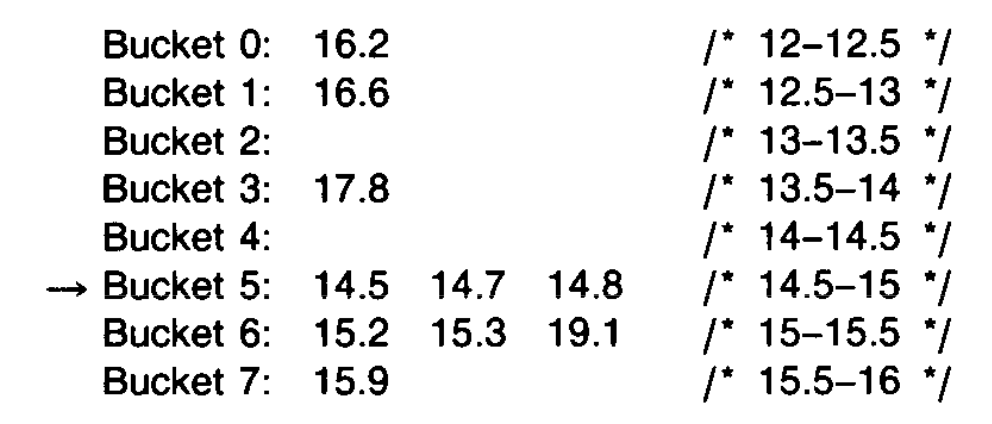
\includegraphics[width=0.4\textwidth]{images/cq}\caption{Calendar Queue - Struktur \cite{brown_cq}}\label{Calendar Queue - Struktur}
	Beispiel einer Calendar Queue mit Bucketbreite 0.5 und Jahresl�nge 8. Das Event zur Zeit 19.1 wird beim \textit{dequeuen} in diesem Jahr �bersprungen.
\end{figure}
\subsection{Optimierungen}
Die L�nge eines Jahres und die L�nge eines Tages werden dynamisch an die Anzahl der Events angepasst. Steigt die Zahl der Events auf mehr als das doppelte der Anzahl der Buckets, werden die Events in eine \ac{CQ} doppelter Gr��e kopiert, sodass durchschnittlich jedes Event in einem eigenen Bucket liegt. Analog halbiert sich die Gr��e der \ac{CQ} bei halb so viel Events wie Buckets in der \ac{CQ} vorhanden sind. Die \textit{\aclu{bw}} wird beim Vergr��ern/Verkleinern angepasst. Sie sollte ungef�hr so gro� sein, wie die durchschnittliche Zeit zwischen zwei benachbarten Events.
Eine von Brown vorgeschlagene Heuristik, eine akzeptable \textit{\acl{bw}} zu ermitteln, ist, die ersten \textit{n} Elemente zu \textit{dequeuen}, die durchschnittliche Zeit zwischen diesen Events zu errechnen, und diese anschlie�end wieder zu \textit{enqueuen}. In Bezug auf statistische Aussagekraft muss \textit{n} hinreichend gro� gew�hlt werden. \cite{brown_cq}
\subsection{Performance}
Die Calendar Queue hat eine theoretische Komplexit�t von $ O(1) $ f�r sowohl die \textit{dequeue}- als auch die \textit{enqueue}-Operation. 
Die amortisierte Zeit wird jedoch ma�geblich durch die Zeitverteilung der Events beeinflusst. W�hrend die Performance bei absoluter Gleichverteilung optimal ist, ist bei gro�er Varianz des Abstandes der Events zueinander keine konsistente Performance gegeben. Wenn sich Events innerhalb eines Buckets h�ufen, dauert das \textit{enqueuen} l�nger, da die \ac{LL} l�nger wird. Wenn viel Zeit zwischen den Events liegt, m�ssen viele leere Buckets untersucht werden, bevor das n�chste Element gefunden wird.  \cite{brown_cq}\cite{wuttisittikulkij_study_2003} \\
Brown schl�gt zur Behebung letzteren Problems eine Strategie vor, nach der nach einem eventfreien Jahreszyklus das kleinste Element von allen Buckets zur�ckgegeben wird. \cite{brown_cq}
\subsection{Erweiterung: Dynamic Calendar Queue}
In der \ac{DCQ} wird die Heuristik zur Berechnung von \textit{\ac{bw}} beim Kopieren in eine gr��ere bzw. kleinere Queue ver�ndert. Es werden nicht die ersten \textit{n} Elemente zur Berechnung der durchschnittlichen Zeit zwischen den Events genutzt, sondern Elemente aus dem Bucket, in dem die meisten Events sind. So soll ein repr�sentativeres Ergebnis der Zwischeneventzeit erzielt werden.
Au�erdem werden zwei Metriken eingef�hrt: Die durchschnittlichen \textit{enqueue}- und \textit{dequeue}-Kosten ($C_E$ und $C_D$). Wenn diese einen vorher definierten Grenzwert �berschreiten, wird eine Neuberechnung von \textit{\ac{bw}} initiiert, sodass sich die Queue an �nderungen in der Eventdistribution \textit{dynamisch} anpasst. \cite{dcq}\cite{snoopy}


\section{MList}
Die \ac{MList} ist eine mehrstufige \ac{PQ}-Implementation, welche auf allen Ebenen \acp{LL} verwendet.

Die MList besteht aus drei Ebenen:
Die unterste Ebene (T3) ist eine �berschussliste f�r Elemente in entfernter Zukunft. Dies ist eine einfache \ac{LL} von Elementen.
Auf zweiter Ebene (T2) gibt es eine \ac{LL} von Buckets gleicher Breite. Die Buckets sind monoton fallend nach Priorit�ten sortiert ($ \forall x\in B_i,y \in B_{i+1}\colon x\leq y$). Die Elemente innerhalb eines Buckets sind unsortiert in einer \ac{LL} gespeichert.

Auf der h�chsten Ebene (T1) befinden sich die Elemente des aktuellen Buckets in einer sortierten \ac{LL}. \cite{li_mlist}

\begin{figure}[htb]
	\centering
	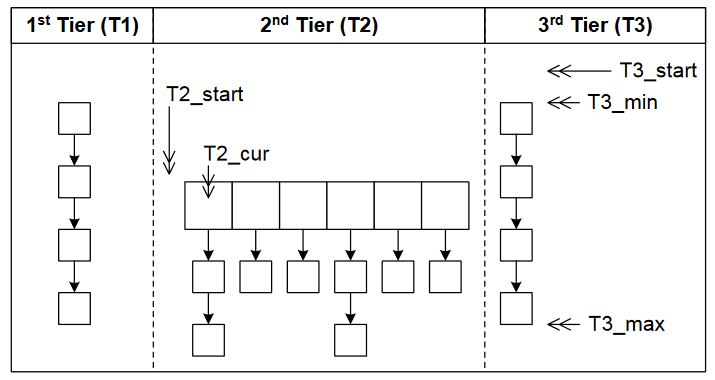
\includegraphics[width=0.4\textwidth]{images/mlist_structure}\caption{Struktur MList \cite{li_mlist}}\label{MList-struktur}
\end{figure}

In T2 wird \textit{\ac{bw}} wie folgt berechnet: 
\begin{equation}
	T2\_bw = \frac{T3\_max - T3\_min}{T3\_count}
\end{equation}

Die Ober- bzw. Untergrenze der Priorit�ten in T3 wird durch \textit{T3\_max} resp. \textit{T3\_min} gegeben; \textit{T3\_count} ist die Anzahl der Elemente in T3.
Die h�chste Priorit�t in T3 wird von \textit{T3\_start} angegeben. Analog dazu ist \textit{T2\_start} die h�chste Priorit�t aus T2.
Der aktuell kleinste nichtleere Bucket in T2 wird durch \textit{T2\_cur} markiert. Werden die Elemente eines Buckets nach T1 �berf�hrt, zeigt \textit{T2\_cur} auf den nachfolgen Bucket in T2.

\subsection{Dequeueing}
Initial ist ausschlie�lich T3 bef�llt. Beim ersten \textit{Dequeue} werden alle Elemente nach T2 verschoben und in Buckets eingeordnet. Anschlie�end werden die Elemente im ersten Bucket (bzw. \textit{T2\_cur}) sortiert und nach T1 verschoben. Ist in einem Bucket nur ein Element, braucht dieses nicht nach T1 verschoben werden, sondern kann direkt zur�ckgegeben werden.
Wenn T1 leer ist, wird der n�chste nicht leere Bucket nach T1 �berf�hrt. Wenn T2 leer ist, werden die zuvor benannten Schritte wiederholt. Das \ac{PES} ist leer, wenn alle Ebenen leer sind.

\subsection{Enqueueing}
Beim \textit{Enqueueing} wird durch die Ebenen T3 bis T1 durchgegangen, um den Einf�gepunkt zu ermitteln. Sobald dieser gefunden ist, kann abgebrochen werden.
F�llt das Element in den Bereich von T3, d.h. wenn es gr��er oder gleich \textit{T3\_start} ist, wird es an das Ende der \ac{LL} geh�ngt.
Andernfalls wird gepr�ft, ob die Priorit�t niedriger als \textit{T2\_cur} ist. Trifft dies zu, wird das Element in den Bucket mit Index \textit{bucket\_idx}, gem�� Gleichung \ref{MList-bucket-index} eingef�gt.
Falls dies nicht zutrifft, wird das Element in T1 einsortiert.\cite{li_mlist}


\begin{equation}
	bucket\_idx = \frac{priority - T2\_start}{T2\_bw}\label{MList-bucket-index}\hspace{1em}vgl. \cite{li_mlist}
\end{equation}

\subsection{Performance}
Die \ac{MList} ist so entworfen, dass bei jedem Sortiervorgang in T1 m�glichst wenige Elemente sortiert werden m�ssen.
Die amortisierte Zeit f�r das \textit{Dequeue} ist nach Li und Thng bei $O(1)$, da die Zeit f�r das Sortieren von wenigen Elementen vernachl�ssigbar ist. \cite{li_mlist}
Weil die \ac{LL} bei jeder �berf�hrung von T2 nach T1 sortiert werden muss, ist die theoretische Zeitkomplexit�t die des genutzten Sortieralgorithmus. 

Da in T2 die Elemente nur in Buckets eingeordnet werden, ist dies weniger aufwendig, als ein vollst�ndiger Sortiervorgang. \cite{li_mlist}
In \cite{bucket-sort} wird geschrieben, dass die Zeitkomplexit�t von \textit{Bucket Sort} bei $O(n)$ liegt. Jedoch auch, dass andere Algorithmen f�r besonders kleine oder besonders gro�e Listen �hnlich schnell oder schneller sind.

In T3 wird nicht sortiert, sondern immer am Ende angef�gt. Daraus ergibt sich $\Theta (1)$ f�r das Einf�gen auf dieser Ebene.

%\begin{figure}[htb]
%    \centering
%    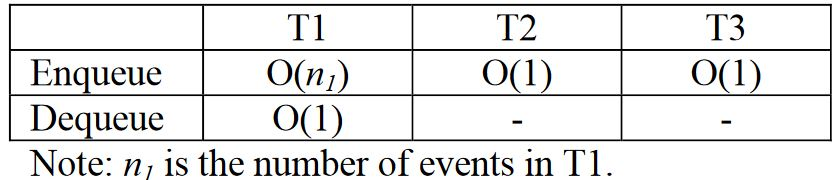
\includegraphics[width=0.7\textwidth]{images/mlist_complexity}\caption{Amortisierte Zeitkomplexit�t der MList Operationen \cite{li_mlist}}\label{MList-complexity}
%\end{figure}


Unter Verwendung von Alternativen zur \ac{LL} kann u.U. bei der �berf�hrung von einer Ebene in die n�chste ein Performancegewinn erzielt werden. \cite{exp-s-t}\cite{deterministic-sorting}

\section{Fazit}
%Die Performanceverbesserung des Parallel Heap gegen�ber dem klassischen Heap stammt nicht von einer anderen Laufzeitkomplexit�tsklasse, sondern von der parallelen Verarbeitung der Elemente.
%Entsprechend sind die theoretische und amortisierte Zeitkomplexit�t gleich denen des Heaps.
Der \textit{Parallel Heap} eignet sich nur bedingt f�r die \textit{diskrete eventbasierte Simulation}, da durch die parallele Verarbeitung der Elemente eine Wiederholbarkeit der Ergebnisse nicht garantiert ist.
Die \textit{\ac{CQ}} ist eine Verbesserung gegen�ber der \textit{\ac{PQ}}, kann jedoch bei ungleich verteilten Events nicht mit der \textit{\ac{MList}} mithalten.

	\begin{table}[hb]
	\resizebox{0.8\textwidth}{!}{
		\begin{minipage}{\textwidth}
			\begin{tabular}{|c|c|c|c|c|}
			\hline  & PQ(Heap) & Parallel Heap & CQ & MList \\ 
			\hline Theoretisch enqueue & $ O(log n) $ & $ O(log n) $ & $ O(1) $ & $ O(n_1) $ \footnote[1]{$ n_1 $ sei die Anzahl der Elemente in T1} / $ O(1) $ \\ 
			\hline Theoretisch dequeue & $ \Theta(log n) $ & $ \Theta(log n) $ & $ O(1) $ & $ O(n log n) $ \footnote[2]{inkl. Kosten der �berf�hrung zwischen den Tiers}/ $ O(1) $ \\ 
			\hline Amortisiert enqueue & $ O(log n) $ & $ O(log n) $ & $ O(1) $ \footnote[3]{Abh�ngig von der Eventverteilung m�glicherweise langsamer} & $ O(n_1)$ \footnotemark[1] / $ O(1) $ \\ 
			\hline Amortisiert dequeue & $ \Theta(log n) $ & $ \Theta(log n) $ & $ O(1) $ \footnotemark[3] & $ O(1) $ \\ 
			\hline 
			\end{tabular}
		\caption{�bersicht Laufzeitkomplexit�ten}
		\end{minipage}
	}
	\end{table}

\textbf{Somit ist die \textit{\ac{MList}} zur Reduktion des \textit{\ac{PES}-Problems} unter den verglichenen Implementationen die beste Wahl. }


\begin{acronym}[UML]
\acro{DES}{Diskrete Eventbasierte Simulation}
\acro{FIFO}{First In First Out}
\acro{CQ}{Calendar Queue}
\acro{DCQ}{Dynamic Calendar Queue}
\acro{PQ}{Priority Queue}
\acro{LL}{Linked List}
\acro{MList}{Multi-tier Linked List}
\acro{bw}{bucket width}
\acro{PES}{Pending Event Set}
\end{acronym}

\clearpage
\bibliography{aktemplate}
\end{document}
